\documentclass[a4paper]{article}
\usepackage[utf8]{inputenc}
\usepackage[french]{babel}
\usepackage[T1]{fontenc}
\usepackage{graphicx}
\usepackage[a4paper,top=3cm,bottom=2cm,left=3cm,right=3cm,marginparwidth=1.75cm]{geometry}
\usepackage[colorlinks=true, allcolors=blue]{hyperref}

\usepackage{fancyvrb}
\usepackage{listings}
\usepackage{color}
\definecolor{dkgreen}{rgb}{0,0.6,0}
\definecolor{gray}{rgb}{0.5,0.5,0.5}
\definecolor{mauve}{rgb}{0.58,0,0.82}
\lstset{frame=tb,
  language=Java,
  aboveskip=3mm,
  belowskip=3mm,
  showstringspaces=false,
  columns=flexible,
  basicstyle={\small\ttfamily},
  numbers=none,
  numberstyle=\tiny\color{gray},
  keywordstyle=\color{blue},
  commentstyle=\color{dkgreen},
  stringstyle=\color{mauve},
  breaklines=true,
  breakatwhitespace=true,
  tabsize=3,
  inputencoding=utf8
}

\title{VisualImpro : Documentation}
\author{Alexandre Casanova--Franger\and
Gauthier Lamarque\and Paul Simorre\and Lucas Vivas}
\begin{document}
\maketitle

\tableofcontents

\section{Introduction} \paragraph{Ce document vise à présenter et documenter le
projet d’outil d’improvisation musicale intégré à la plateforme Bela dont le
développement a commencé en Juin 2017. Nous décrirons son fonctionnement en
détail aussi bien pour l’utilisateur que le programmeur, ainsi que les
possibilités d’amélioration pour un développement ultérieur. Avant de continuer,
il est conseillé de s’informer sur les généralités concernant le Bela (son
fonctionnement, ses entrées/sorties, etc) ainsi que le capelet additionnel pour
les entrées audio sur le \href{https://github.com/BelaPlatform/Bela/wiki}{wiki}
de bela.io .}

\section{Présentation générale du projet} \paragraph{Le projet consiste en la
création d’un outil pour l’improvisation musicale, permettant à des musiciens de
jouer tout en ayant en même temps une retrospective visuelle et sonore en temps
réel de leur improvisation. Cette représentation permet notamment de visualiser
les paires de corrélations entre les musiciens deux à deux. Formellement, elle
se résume à la chose suivante :} \

\begin{Verbatim}
Entrée : N pistes musicales (musiciens et/ou pistes enregistrées)
Sortie : une matrice M de taille NxN,
	où M(i,j)=M(j,i) est la corrélation des pistes i et j.
\end{Verbatim}

\paragraph{Cette matrice doit se mettre à jour régulièrement et en temps réel.
De plus, la notion de "corrélation" étant large et subjective, on souhaitait
pouvoir changer de fonction de corrélation facilement selon les besoins. La
décision d’utiliser comme support la plateforme Bela est justifiée car elle
comprend un grand nombre d’entrées/sorties audio, ce qui est idéal pour ce
projet. Finalement les objectifs visés sont les suivants :}

\begin{itemize} \item proposer une visualisation simple de la matrice (sur une
page web) \item rendre simple le changement des algorithmes de traitements
visuel et sonores \item permettre la possibilité d’ajouter des effets audio
avant calcul \item obtenir un retour sonore en temps réel correspondant à un
calcul de corrélation entre les musiciens \end{itemize}

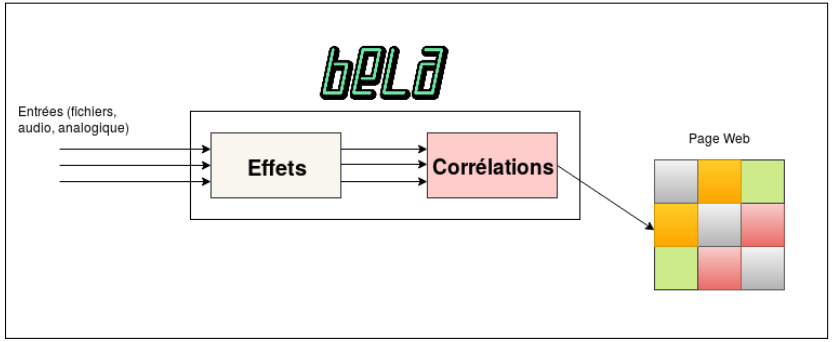
\includegraphics[width=1\textwidth]{Bela1.png}

\section{Utilisation} \paragraph{Cette partie explique comment utiliser le
logiciel. Il existe deux manières de le lancer, toutes deux en ligne de
commande, l’une depuis la session utilisateur et l’autre en ssh depuis Bela.}

\subsection{Depuis l'ordinateur} \paragraph{Cette méthode est la plus simple
pour les néophytes car elle est opaque. Pour utiliser cette méthode, il suffit
d’avoir un PC sous Linux avec le logiciel nodejs installé. Tout d’abord,
dézippez le fichier VisualImproExe.zip . Vous allez vous retrouver avec un
dossier VisualImproExe sur votre ordinateur, contenant tout le nécessaire pour
lancer le projet. Rendez vous dans ce dossier en ligne de
commande.\newline\newline}

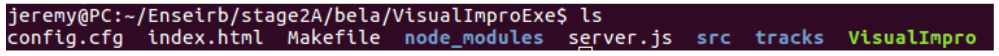
\includegraphics[width=1\textwidth]{terminal1.png}

\paragraph{Ce dossier contient deux fichiers importants pour l’utilisateur : le
fichier de configuration config.cfg, et exécutable VisualImpro. Le fichier
config.cfg sert à configurer le programme avant son exécution. Vous pouvez ici
choisir les fichiers que vous voulez ajouter en spécifiant leur chemin, ainsi
que le nombre de pistes audio (2 pistes max, qui correspondent aux entrées audio
de l’étage du bas), de pistes analogiques (8 entrées sur l’étage supérieur du
Bela), ainsi que les 4 fonctions de calcul utilisées (ces fonctions seront
détaillées plus tard). Vous pouvez enfin choisir la taille des buffers de calcul
et choisir d’activer les effets ou non. Tous les paramètres sont expliqués en
commentaire dans le fichier. Configurez le fichier comme nécessaire. Vous pouvez
ajouter les fichiers wav que vous souhaitez utiliser dans le dossier tracks pour
plus de simplicité. Les fichiers wav que vous utilisez devront être
échantillonnés à 44100 Hz (sinon la vitesse de lecture sera inadaptée). Une fois
le fichier configuré et sauvegardé, vous pouvez lancer le programme. Lancez en
ligne de commande ./VisualImpro depuis le répertoire VisualImproExe/. Cette
commande démarrera automatiquement le serveur, le programme sur Bela et la page
web.}

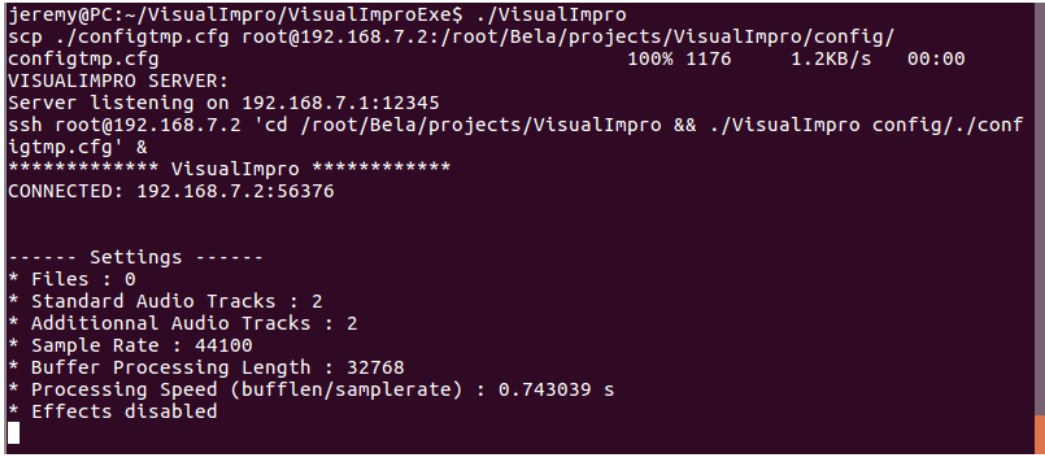
\includegraphics[width=1\textwidth]{terminal2.png}

\paragraph{Vous pouvez ensuite, si ce n’est déjà fait, brancher vos entrées
monopistes sur le Bela. Les entrées disponibles seront toujours dans l’ordre
croissant. Par exemple, si vous avez décidé d’activer 5 entrées analogiques,
seules les entrées numérotées de 0 à 4 seront disponibles. Les autres sont
désactivées. Vous pourrez ensuite observer, après lancement du programme, la
matrice de corrélation des signaux que vous avez passés en entrée. Lorsque vous
voudrez arrêter le programme, appuyer sur Ctrl+C dans le terminal ouvert. Cette
commande stoppe le programme et supprime les fichiers wav du Bela. Vous aurez
ensuite accès, dans le dossier logs, à un enregistrement en texte des matrices
de corrélation successives. Ces fichiers sont nommés par la date et l’heure de
fin du programme.}

\subsection{En ssh depuis Bela} \paragraph{Cette utilisation est plus compliquée
mais il est utile de la connaitre pour un programmeur. Vous devrez d’abord
ouvrir 2 terminaux sur lesquels vous vous connecterez en ssh sur
Bela.\newline\newline}

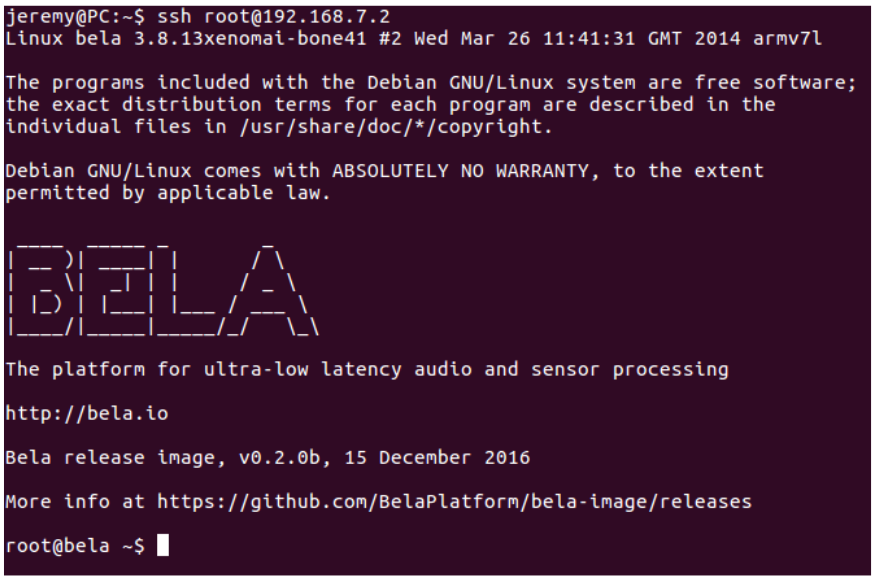
\includegraphics[width=1\textwidth]{terminal3.png}

\paragraph{Dans le premier terminal, rendez vous dans le repertoire
~/Bela/IDE/public/VisualImpro. Tapez ensuite la commande node server.js. Cette
commande démarre le serveur communiquant entre la page web et le programme.
Ouvrez ensuite une page web à l’adresse 192.168.7.2:8080. Ceci correspond à
l’adresse IP de Bela et le port du programme utilisé. Enfin, dans le second
terminal, rendez vous dans le dossier ~/Bela/projects/VisualImpro. Modifiez
ensuite le fichier settings.cfg, de la même manière que le fichier config.cfg de
la première méthode. Vous devrez importer vos fichier wav manuellement, ou via
l’IDE Bela à l’adresse 192.168.7.2 (visitez le wiki de bela.io pour plus
d’informations). Enfin, lancez la commande ./VisualImpro. Le programme se lance.
Pour arrêter le programme vous devrez tout fermer à la main. A la fin du
programme, les résultats sont stockés dans le fichier log/log, cependant on ne
conserve pas de trace des précédents résultats. Cette méthode est plus
compliquée mais utile pour un développeur, car plus rapide et plus transparente
que la première (il n’y a pas de transfert de fichiers wav donc plus rapide). Il
est possible de laisser tourner le serveur et la page web et de ne relancer que
le programme à chaque fois. Il est aussi possible de lancer le programme via
l’IDE plutôt qu’en ligne de commande, en spécifiant les bons flags au
compilateur si vous recompilez. Pour compiler le programme en ssh, il faudra
vous rendre dans le dossier \textasciitilde/Bela, et taper en ligne de commande
\textit{make PROJECT=VisualImpro LDLIBS=-ldl}. Pour clean le dossier il faudra
exécuter \textit{make projectclean PROJECT=VisualImpro}. Pour toute autre
spécification concernant la compilation, vous pourrez utiliser \textit{make
help} pour obtenir de l'aide.}

\subsection{Ajouter des plug-ins de traitement de la matrice} \paragraph{Le
calcul de la matrice peut se configurer à l’exécution comme nous l’avons vu. Il
est de plus possible de rajouter des plug-in de calcul au programme. Ces
fonctions se répartissent en quatre catégories, et correspondent au quatre
étapes de calcul du programme :}

\begin{itemize} \item les fonctions de "pre-processing", traitement du signal
d’entrée en amont \item les fonctions de calcul de coefficient de corrélation
\item les fonctions associant un coefficient à une couleur. \item les fonctions
de traitement du son par rapport à la corrélation entre les musiciens
\end{itemize}

\paragraph{Pour ajouter une fonction, votre fichier devra respecter les critères
suivants :}

\begin{itemize} \item il devra s’appeler Preproc*.cpp, Coeff*.cpp, Color*.cpp ou
Mix*.cpp selon que vous ajoutiez une fonction de preprocessing, de corrélation,
de couleur ou de mixage. \item les fonctions ajoutées devront respecter les
prototypes standards exposés plus bas. \end{itemize}

\paragraph{Enfin, le fichier placé dans le répertoire process devra respecter le
squelette suivant :}
\

\begin{lstlisting}
#include "../utilities.cpp" //pour inclure la structure
Triplet // code de fonctions auxiliaires
extern "C"{ // code de ma fonction
Preproc, Color ou Coeff
}
\end{lstlisting}

\paragraph{De plus, pour tester votre fonction avant de l’ajouter au programme,
vous aurez besoin de la classe Triplet :}
\

\begin{lstlisting}
class Triplet{
	public:
		int one, two, three;
	Triplet(int _one, int _two, int _three) : one(_one), two(_two), three(_three){} };
\end{lstlisting}

\paragraph{Ce triplet correspond à un triplet RGB. Les entiers contenus sont
donc entre 0 et 255, one étant le rouge, two, le vert et three le bleu.}
\newpage

\subsubsection{Prepoc} \paragraph{Ces fonctions ont le prototype suivant :}
\

\begin{lstlisting}
std::vector<std::vector<float> > PreprocX (const std::vector<std::vector<float> >& buff);
\end{lstlisting}

\paragraph{L’argument en entrée est une matrice de vecteurs représentant les
signaux d’entrée. Ici buff.size() est égal au nombre de pistes, et la longueur
de tous les éléments du tableau (un vecteur) est identique et correspond à la
longueur du signal à traiter en temps réel. La matrice de sortie sera donc de
taille $buff.size() \times x$, où $x$ peut être différent de la longueur des
signaux initiaux. Cette fonction peut correspondre par exemple à :}

\begin{itemize} \item un calcul d’enveloppe du signal \item un filtrage \item
une transformée de fourrier \item un ré échantillonnage \item un autre
traitement quelconque à implémenter \end{itemize}

\paragraph{Par exemple, la fonction PreprocEnergy calcule énergie moyenne du
signal sur des petits intervalles et les vecteurs retournés sont des enveloppes
énergie, de taille bien inférieure à la taille du signal. Il est intéressant de
réduire la taille des signaux d’entrée grâce à ces fonctions, car cela améliore
nettement les performances du programme. Il peut par exemple être judicieux de
créer une fonction qui garde 1 échantillon sur 2, 3 ou 4 de manière à alléger
les calculs de corrélations en suite de chaîne.}

\subsubsection{Coeff} \paragraph{Ces fonctions ont le prototype suivant :}
\

\begin{lstlisting}
float CoeffX (const std::vector<float>& s1, const std::vector<float>& s2);
\end{lstlisting}

\paragraph{Les arguments en entrée sont 2 vecteurs, provenant de la matrice
retournée par la fonction Preproc précédente. Le flottant en sortie correspond à
la corrélation de ces deux signaux. Cette fonction sera appelée
$\frac{n(n-1)}{2}$ fois, où n est le nombre de pistes. La corrélation est
symétrique, entre 0 et 1, et vaut toujours 1 lorsqu’un signal est corrélé à lui
même. La corrélation classique correspond au produit scalaire euclidien.}

\subsubsection{Color} \paragraph{Ces fonctions ont le prototype suivant :}
\

\begin{lstlisting}
Triplet ColorX (float coeff);
\end{lstlisting}

\paragraph{Elle convertit un coefficient de corrélation en une couleur,
représentée par son triplet RGB. Voir les exemples d’échelles ColorBlackToWhite
et ColorGreenToRed déjà implémentés.}

\subsubsection{Mix} \paragraph{Ces fonctions ont le prototype suivant :}
\

\begin{lstlisting}
vector<float> MixMaxCorrelated(const vector<vector<float> >& correlMatrix)
\end{lstlisting}

\paragraph{Cette fonction prend en paramètre une référence d'un vecteur situé
initialement dans render.cpp, qui est notre fichier de traitement principal,
appelé par le main, que nous détaillerons plus tard. On utilise une référence
ici car c'est la seule solution pour renvoyer des valeurs obtenues dans les
tâches auxiliaires à la boucle de traitement principale. Cette fonction va
calculer, dans le cas de base, la moyenne de corrélation de chaque instrument
par rapport aux autres. Cette moyenne peut être calculée selon les paires
d'instruments les mieux corrélés, les moins corrélés, ou encore une fonction
retournant des valeurs aléatoires. Ce dernier cas pourrait être perçu comme un
atout expérimental pour ce projet, qui est un projet de recherche et qui
pourrait mener à d'intéressants résultats. Si l'on ne souhaite pas définir de
fonction de mixage, nous pourrons utiliser la fonction MixNeutral qui renvoie un
vecteur de valeurs neutres, qui n'auront aucun impact sur le volume sonore}

\subsubsection{Ajouter d'autres fonctions} \paragraph{Une fois que votre
fonction est testée, placez-la dans le répertoire process du projet. Dans ce
répertoire, compilez avec make. Vous n’avez alors plus qu’à changer les
paramètres du fichier de configuration que vous utilisez. Par exemple, si vous
avez créé une fonction ColorBlueToYellow, dans un fichier ColorBlueToYellow.cpp,
changez le fichier de configuration en spécifiant COLOR ColorBlueToYellow à la
place de ce qui y est écrit actuellement.}

\section{Généralités sur Bela}

\subsection{Caractéristiques technique} \paragraph{La plateforme embarquée Bela
est idéale pour réaliser ce genre de projets. En effet, elle dispose de
nombreuses entrées audio, analogiques et digitales pour capter les signaux
sonores d’entrée, ainsi que de nombreuses sorties, et se connecte à un PC sous
Linux en branchant un simple cable USB. Il est dès lors très simple de coder sur
Bela, en ssh depuis un terminal par la commande ssh root@192.168.7.2, ou depuis
l’IDE depuis un navigateur à l’adresse \href{http://192.168.7.2/}{192.168.7.2}
(accessible sans connexion internet). D’autres informations sont disponibles sur
le \href{https://github.com/BelaPlatform/Bela/wiki}{wiki} de Bela.}

\subsection{Structure d'un projet Bela en C++} \paragraph{Voir la
\href{https://github.com/BelaPlatform/Bela/wiki/Example-projects-and-tutorials}{documentation}
de \textit{bela.io}. Le projet d’improvisation musicale a été implémenté en C++.
Un projet se crée via l’IDE ("new project"). Il correspond à un dossier
contenant au moins un fichier, le fichier render.cpp. Ce fichier contient lui
même 3 fonctions :}

\begin{itemize} \item setup() appelée avant le démarrage de l’audio. Elle
initialise les ressources et leur alloue de la mémoire. C'est la fonction qui
effectuera de gros calculs avant le démarrage des tâches. \item render() est
appelée lors du processus audio. Elle est appelée régulièrement, à chaque fois
qu’un nouveau bloc audio est disponible, avec une priorité supérieure à toutes
les autres taches sur le processeur. Chaque fois qu’elle est appelée, elle
dispose en argument de buffers contenant les échantillons à traiter. \item
cleanup() est appelée à la fin du processus et libère éventuellement les
ressources allouées, termine des tâches, etc. \end{itemize}

\paragraph{Ces fonctions prennent toutes les mêmes arguments :}

\begin{itemize} \item BelaContext * context, une structure contenant tous les
paramètres du programme, notamment les buffers audio et analogiques. \item void
*userData, un pointeur laissé à disposition du programmeur pour communiquer des
données entre les différentes fonctions. Pour le projet, nous l’utiliserons
notamment pour transferer des paramètres de configuration du main à la fonction
setup, contenus dans une structure ChSettings. \end{itemize}

\paragraph{Compte tenu de la régularité des appels de render, il est important
de veiller à ce que seules les tâches les plus importantes soient exécutées dans
cette fonction. En effet, si une tâche trop coûteuse en temps est présente dans
la fonction, render risque de ne pas finir à temps avant l’arrivée des prochains
échantillons, certains blocs seront donc manqués. Ainsi lorsqu’on aura besoin
d’exécuter des fonctions coûteuses, on les exécutera dans des tâches
auxiliaires. Il est possible d’en créer grâce à la structure AuxiliaryTask et
aux fonctions associées. Voir la doc ici ainsi que les programmes d’exemple Bela
et le code du projet. Enfin, le programme contient un fichier main.cpp. Si aucun
fichier main n’est créé, alors le Makefile spécifie lui même un main par défaut.
Pour notre part, nous avons eu besoin de créer un main plus complexe que
l’original.}

\subsection{Compiler et exécuter un programme Bela} \paragraph{Comme énoncé plus
haut, pour compiler un projet Bela depuis un terminal, se rendre dans le
répertoire ~/Bela, et utiliser make PROJECT=VisualImpro. De plus il est
nécessaire de spécifier certains flags et librairies, par exemple la librairie
dl pour dlopen(). On compile donc par la ligne make PROJECT=VisualImpro
CPPFLAGS=-g LDLIBS=-ldl . Il est aussi possible de compiler depuis l’IDE en
spécifiant les flags dans les paramètres.}

\section{Structure globale du projet} \paragraph{Nous allons présenter dans
cette section le fonctionnement global du programme, sans rentrer dans les
détails. Ce fonctionnement se repose principalement sur les fichiers render.cpp
et main.cpp.}

\subsection{Le fichier main.cpp} \subsubsection{Récupération du fichier de
configuration} \paragraph{On commence d’abord par parser le fichier de
configuration, contenant divers paramètres tels que les noms des fichiers audio à
charger, le nombre d’entrées analogiques, etc. Si aucun argument n’est spécifié
au programme, on charge le fichier settings.cfg sur le Bela. Sinon, l’argument
fixe le fichier à charger. On récupère les données de ce fichier grâce à la
classe Parser, et on stocke ces paramètres dans une structure ChSettings. Cette
structure sera ensuite communiquée au thread audio. On récupère notamment les
fonctions de la libraire libprocess.so créée dans le dossier process, grâce à
dlopen.}

\subsubsection{Initialiser les paramètres audio} \paragraph{Cette partie du main
est semblable à celle du main par défaut. Elle sert à initialiser le thread
audio via les fonctions Bela\_initAudio(), Bela\_defaultSettings(),
Bela\_startAudio() et tous les traitements faits autour de ces fonctions. Voir
un exemple de main classique dans un autre projet
\href{https://github.com/BelaPlatform/Bela/blob/master/examples/07-DataLogging/logging-sensors/main.cpp}{ici}.
On commence par initialiser la variable settings qui contient les paramètres
audio (nombre de canaux analogiques, etc). On l’initialise avec les paramètres
par défaut avec Bela\_defaultSettings(), puis on règle le nombre de canaux
analogiques comme définis dans le fichier de configuration. Dans le main par
défaut, settings est modifié grâce aux paramètres en ligne de commande. Pour
éviter de modifier en dur cette variable, et risquer d’oublier un paramètre,
nous avons créé des variables argc et argv similaires aux arguments du main,
avec les paramètres à modifier. ces variables sont ensuite passées en arguments
de Bela\_getopt\_long(), qui parse ces variables et modifie settings en
conséquence. En l’occurence, nous spécifions le nombre de pistes analogiques à
utiliser (-C 4 ou 8), ainsi que celles à activer (-Y). Enfin, la fonction
Bela\_initAudio() récupère les paramètres via la variable settings. Ces
paramètres seront utilisables dans les fonctions de render.cpp via l’argument
userData.}

\subsection{Le fichier render.cpp}

\subsubsection{La fonction setup()} \paragraph{La fonction récupère les
paramètres passés par le main via l’argument userData, et les stocke dans des
variables globales. Elle initialise notamment les structures permettant de lire
les fichiers wav, ainsi que les buffers pour stocker les échantillons et les
traiter ensuite.}

\subsubsection{La fonction render()} \paragraph{La fonction render suit
globalement le schéma suivant :}

\begin{Verbatim}
pour chaque frame de données :
	avancer le curseur des fichiers de 1
	lancer le calcul de la matrice si les buffers sont remplis
	si effets activés:
		boucle effets
	sinon
		boucle normale
	écrire dans la sortie audio
\end{Verbatim}

\paragraph{Les boucles d’effets et normale seront expliquées plus en détail
ensuite, mais consistent grossièrement à lire dans les entrées standards
(fichiers, analogiques et audio) les échantillons arrivant, et les stocker dans
une matrice de taille \textit{nb\_pistes} $\times$ \textit{taille\_buffer},
représentant les pistes à traiter. La différence entre les deux boucles est que
la boucle d’effets contient un traitement supplémentaire pour calculer les
effets, tandis que la boucle normale stocke directement les échantillons.}

\section{Boucle de traitement de render.cpp} \paragraph{Après avoir expliqué le
fonctionnement global de cette boucle, nous allons nous concentrer sur les
détails, et expliquer chaque ligne de l’algorithme décrit en 5.2.2. Tout
d’abord, on répète la boucle "pour chaque bloc de données". En fait, à chaque
appel de render, l’argument context contient des nouveaux buffers audioIn et
analogIn, contenant les nouveaux échantillons. Ces buffers sont constitués de
frames. Une frame correspond à un nombre d’échantillons égal au nombre de
pistes, et représente chaque signal à un instant t. Les buffers sont constitués
de plusieurs frames, il faut donc répéter le traitement de render autant de fois
qu’il y a de frames.}

\subsection{Curseur des fichiers} \paragraph{Bien que les buffers analogiques et
audio se mettent à jour automatiquement, ce n’est pas le cas des structures
permettant de lire les fichiers, c’est à dire la classe SampleStream. Cette
classe a été créée dans le programme d’exemple sample-streamer-multi et
réutilisée dans ce projet. Elle dispose notamment d’une méthode processFrame(),
permettant simplement d’avancer le curseur de lecture des fichiers. Il est
nécessaire d’adapter la vitesse de lecture à celle des entrées physiques. La
boucle dispose donc d’une instruction appelant la méthode processFrame() pour
chaque piste.}

\subsection{Boucle normale} \paragraph{Cette partie correspond à la ligne
"boucle normale". Elle consiste à récupérer les échantillons des différents
canaux pour les stocker dans des buffers. Ces buffers sont stockés dans la
structure suivante :} \

\begin{lstlisting}
vector<vector<float> > gProcessBuffer;
\end{lstlisting}

\paragraph{La première dimension de cette matrice est le nombre de pistes, et
chaque gProcessBuffer[i] est un vecteur représentant le signal audio, de taille
gUserSet.buffer\_len (initialisé dans setup() et correspondant à un paramètre du
fichier de configuration). Les signaux sont stockés de la manière suivante :}

\begin{itemize} \item de 0 à gN umStreams - 1 : fichiers wav \item de gN
umStreams à gN umStreams + gN umAnalog - 1 : entrées analogiques \item de gN
umStream + gN umAnalog à la fin : entrées audio \end{itemize}

\subsection{Boucle d'effets} \paragraph{Le début de cette boucle est le même que
la boucle normale : les échantillons sont stockés dans une matrice appelé
gEffectBufferIn, de taille fixée par l’utilisateur (EFFECT\_BUFFER\_LEN). De
plus, on a initialisé une autre matrice, gEffectBufferOut, de deuxième dimension
deux fois plus grande. Ce sont les valeurs de cette matrice qui seront utilisés
pour le calcul de la matrice de corrélation et la sortie audio. Les buffers
gEffectBufferIn et gEffectBufferOut suivent le fonctionnement d’un buffer
circulaire. Les échantillons sont donc transferés de premier buffer vers le
second, avec au milieu l’application de l’effet voulu. On initialise aussi des
curseurs :}

\begin{itemize} \item gReadPointer : entier pour savoir où mettre le prochain
echantillon dans gEffectBufferIn \item gWritePointer : entier pour savoir quel
est le prochain échantillon à lire de gEffectBufferOut \item gLastSample :
dernier échantillon valide de gEffectBufferOut \item gIndIn : indice de
gEffectBufferIn à partir duquel le signal doit être traité. Vaut généralement 0.
\item gIndOut : premier indice de gEffectBufferOut non utiisé. On commencera à
copier le signal traité ici. \end{itemize}

\paragraph{Au premier transfert, l’algorithme est le suivant :}

\begin{Verbatim}
si gEffectBufferIn est plein :
	gEffectBufferIn.swap(gEffectBufferInCopy) //on libère BufferIn pour que
    						//les autres samples arrivent
	gWritePointer = 0; //en attendant le calcul, il faut lire les
    			//échantillons à partir de 0
	gIndOut = gEffSize; //on va ecrire le résultat du premier signal
    			//traité à cet indice.
	Bela_scheduleAuxiliaireTask(gEffectTask);
\end{Verbatim}

\paragraph{De cette manière, render va lire gEffSize échantillons vides. Pendant
ce temps, la tâche sera exécutée, et se terminera avant que render ait lu
gEffSize échantillons. Il lira donc les premiers signaux traités normalement.
Par la suite, l’algorithme fait en sorte de copier le résultat au début du
buffer et à la fin alternativement. Pendant ce temps, le buffer est lu de
manière circulaire, c’est à dire que lorsque le curseur de lecture arrive à la
fin du buffer, il retourne au début, et ainsi de suite. Ceci permet de ne pas
causer d’interruption ou de corruption du signal.}

\subsection{Calcul de la matrice} \paragraph{Cette partie de l’algorithme se
rapporte au calcul et à l’envoi de la matrice. Elle s’explique comme ceci :}

\begin{Verbatim}
si gProcessBuffer est plein : copier(gProcessBuffer,
	gProcessBufferCopy); reset(gProcessBuffer);
	lancerTacheAuxiliaire(gProcessBufferTask);
\end{Verbatim}

\paragraph{L’instruction de copie est en fait un swap de deux vecteurs, qui
échange les adresses et se fait en temps constant. Reset revient simplement à
réinitialiser le curseur de position du buffer. Enfin, la tâche auxiliaire est
lancée via \\ Bela\_scheduleAuxiliaryTask(gProcessBufferTask), où
gProcessBufferTask lance une fonction processBuffer() définie préalablement, et
appelant les fonctions de calcul de matrice dont nous parlerons dans la partie
sur la classe ProcessMultiCorrel.}

\subsection{Sortie audio} \paragraph{Pour entendre le résultat final dans le cas
de base, il est nécessaire d’écrire la somme de ces signaux dans une sortie
audio. Pour ce faire, il existe dans la boucle normale et la boucle d’effet une
variable flottante out. Cette variable sert à stocker la somme des signaux à
mesure qu’on les récupère. L'idée est qu'avec l'introduction des fonctions de
mixage nous pourrons multiplier le volume de chaque instrument par la moyenne de
la corrélation de cet instrument par rapport aux autres (valeur comprise entre 0
et 1). Ces moyennes de corrélations sont donc contenues dans le vecteur
gMeanCorrel, et traité en tâche auxiliaire gProcessBufferTask, en même temps que
se fait le calcul de la matrice. On récupérera donc les valeurs de ce calcul en
passant le vecteur par référence. A la fin de la boucle, on écrit la valeur de
out dans les 2 sorties audio, pour avoir une sortie stéréo. On utilise pour cela
la fonction audioWrite détaillée dans la documentation.}

\subsection{Adaptation du taux d'échantillonnage} \paragraph{Enfin, vous pourrez
remarquer dans le code, la présence de certaines instructions if (gSampleFactor ==
STANDARD\_SAMPLE\_RATE) . Ces instructions correspondent à de petits changements
nécessaires lorsque le taux d’échantillonnage des entrées analogiques varie. En
effet, Bela impose d’utiliser soit 4 sorties analogiques à 44100 Hz, soit 8
sorties analogiques à 22050 Hz. Dans le premier cas, il n’y a pas de problème.
Mais dans le deuxième cas, des modifications sont nécessaires. En effet, les
entrées audio classiques ainsi que les fichiers ne peuvent pas choisir leur
fréquence d’échantillonnage, celle ci étant fixée à 44100 Hz. Il est donc
nécessaire d’adapter artificiellement les entrées audio et fichiers. Dans les
deux cas, cela revient à récupérer un échantillon sur deux. Pour gérer les
fichiers, il est nécessaire de faire défiler le curseur 2 fois plus vite : ceci
explique la présence d’une deuxième instruction processFrame() dans le cas ou on
est à 22050 Hz, qui bouge le curseur une fois supplémentaire. Pour les entrées
audio, il faut simplement lire une fois sur deux, d’où le audioRead(context,
2*n, a) à 22050 Hz. Enfin, la sortie audio est elle-même échantillonnée à 44100
Hz. Lorsqu’on choisit un taux à 22050 Hz, il faut écrire deux fois plus
d’échantillons que ce qu’on a dans les buffers, de manière à rééchantillonner
artificiellement. On écrit donc 2 fois de suite la même valeur en sortie. Ces
modifications permettent donc à l’utilisateur de choisir le nombre de pistes
analogiques dont il a besoin sans se préoccuper du traitement. Lorsqu’il choisit
entre 0 et 4 entrées analogiques, gSampleFactor vaut 2, ce qui correspond à
44100 Hz. Si il choisit 5 entrées ou plus, gSampleFactor vaut 1 pour 22050 Hz.}

\subsection{Autres remarques} \paragraph{Il existe aussi avant la boucle
principale, une instruction \\ Bela\_scheduleAuxiliaryTask(gFillBuffersTask). Celle
ci permet de mettre à jour les buffers liés aux fichiers si besoin. Pour tenter
de gagner de la rapidité, nous avons rajouté un compteur fixé à 10, permettant
d’éviter d’exécuter cette tâche trop souvent. Cependant l’instruction if
entourant cette tâche peut être supprimée sans problème.}

\section{Fichier de configuration} \paragraph{Cette section détaille le
fonctionnement du fichier de configuration, ou plus justement du parser de ce
fichier. Comme dit dans la partie sur le fonctionnement du main, ce parser est
appelé à son début.}

\subsection{Fichier parse.cpp} \paragraph{Nous avons tout d’abord créé un
certain nombre de fonctions de parsing réutilisables dans d’autres cas. Ces
fonctions sont placées dans le fichier parse.cpp :}

\begin{itemize} \item des fonctions is\_number(), is\_ip(), is\_name() ...
permettant de tester un string. \item des fonctions get\_next\_*, prenant en
paramètre en itérateur de string, le modifiant et retournant un string.
\end{itemize}

\paragraph{On utilisera plus tard la fonction get\_next\_word() fonctionnant
comme ceci :}

\begin{verbatim}
string str = "hello world"; string::iterator it = str.begin();
cout << get_next_word(&it); //retourne "hello"
cout << get_next(&it); //retourne " " (espace)
cout << get_next_word(&it); //retourne "world"
\end{verbatim}

\subsection{Fichier Parser.cpp} \paragraph{Cette classe possède des attributs
privés correspondant aux paramètres à récupérer dans le fichier, des getters,
ainsi qu’une méthode get\_word() et un constructeur. get\_word() prend en
paramètre un string et renvoie le deuxième mot. Enfin, le constructeur ouvre le
fichier de configuration, le parcourt ligne par ligne, puis, à l’aide de la
méthode précédente, stocke les paramètres de configuration.}

\subsection{Configuration à l'exécution dans le main} \paragraph{Comme expliqué
dans la partie sur le main, le parser récupère les paramètres du fichier de
configuration à l’exécution. Ces paramètres sont ensuite stockés et interprétés
dans le main puis utilisés dans render.cpp.}

\section{Classe ProcessMultiCorrel} \paragraph{Cette section détaille le
fonctionnement de la classe permettant le calcul de matrices, et plus
généralement le traitement des buffers.}

\subsection{Processing} \paragraph{Lorsqu’on ordonnance la tâche de calcul de la
matrice comme expliqué dans la partie sur render.cpp, la fonction exécutée par
celle ci est la suivante :}

\begin{Verbatim}
ProcessMultiCorrel * p; void processBuffer(){
	if (gBufferProcessed == 0){
    	p->process(gProcessBufferCopy, gUserSet.conn);
    	gBufferProcessed = 1;
	}
}
\end{Verbatim}

\paragraph{Tout le calcul se fait donc par cette méthode process() de la classe
ProcessMultiCorrel. Cette classe contient une méthode process() qui prend en
argument la matrice contenant les signaux, une référence vers le vecteur qui
contiendra les moyennes de corrélation lors du calcul, ainsi qu’un attribut de
la classe Connection permettant de communiquer avec une page web. Cette classe
sera détaillée dans la section à son nom. Cette classe permet véritablement le
calcul de la matrice. Son constructeur prend en paramètre 3 pointeurs de
fonctions, qui correspondent aux fonctions que l’on peut ajouter dans la
librairie process/libprocess.so :}

\begin{itemize} \item une fonction de preprocessing \item une fonction de calcul
de corrélation \item une fonction de mixage, calculant les moyennes de
corrélations \item une fonction associant un coefficient de corrélation à une
couleur pour chaque case de la matrice. \end{itemize}

\paragraph{La méthode process() exécute alors ces fonctions à la suite, afin
d’obtenir notamment une matrice de triplets correspondant à des couleurs. Cette
matrice est alors envoyée via une socket au serveur web (nous détaillerons ce
point dans les sections dédiées).}

\subsubsection{Fichier log} \paragraph{De plus, la méthode enregistre les
valeurs des coefficients de corrélation au fur et à mesure dans le fichier
log/log. Un fichier log se présente sous cette forme :}

\begin{verbatim}
BUFFERSIZE : X SAMPLE_RATE : Y m[1][0] m[2][0] m[2][1] m[3][0]
m[3][1] m[3][2] ... m[n][n-1] m[1][0] m[2][0] m[2][1] m[3][0] m[3][1] m[3][2] ...
m[n][n-1] m[1][0] m[2][0] m[2][1] m[3][0] m[3][1] m[3][2] ... m[n][n-1]
\end{verbatim}

\paragraph{Chaque ligne de coefficient représente une matrice de corrélation.
Pour éviter de stocker l’information redondante, on ne stocke que la partie
basse de la matrice, sans la diagonale.}

\section{Choix des process à l'exécution} \paragraph{Nous avons de plus ajouté
la possibilité de choisir les fonctions précédentes à l’exécution.}

\subsection{Création de la librairie libprocess.so} \paragraph{La librairie
libprocess.so est une bibliothèque dynamique stockant les fonctions créées par
l’utilisateur. Sous réserve que ces fonctions soient correctes et correspondent
aux standards exigés dans le tutoriel du début de cette documentation, cette
librairie se compile via un simple Makefile présent dans le dossier. Il compile
l’ensemble des fichiers concernés :} \

\begin{lstlisting}
g++ -shared -O3 -fPIC Preproc*.cpp Coeff*.cpp Color*.cpp -o libprocess.so
\end{lstlisting}

\paragraph{Les options fPIC et shared permettent de créer le .so, et l’option
-O3 permet de compiler avec le plus d’optimisations possibles. Sans cette
option, le programme est beaucoup plus lent.}

\subsection{Linkage dynamique avec dlopen} \paragraph{Les fonctions définies
dans le fichier de configuration sont ensuite chargées dans le main avec dlopen.
Cette librairie très simple d’utilisation permet de charger dynamiquement les
fonctions d’une librairie. Pour que les noms de symboles correspondent aux noms
de fonctions, il est nécessaire que les fonctions soient implémentées avec
extern "C" comme expliqué dans le tutoriel.}

\section{Serveur web} \paragraph{Cette section détaille le fonctionnement de la
communication entre le programme et la page web.}

\subsection{Classe Connection} \paragraph{Comme expliqué plus haut, les méthodes
process() prennent en argument une instance Connection. Cette classe permet la
communication avec le serveur web via une socket TCP.} \

\begin{lstlisting}
class Connection{
	private :
    	int sockfd;
        bool _isConnected;
		int _port;
        std::string _addr;
	public :
    	Connection() : _port(12345), _addr("192.168.7.1") {}
        Connection(int port, std::string addr) : _port(port), _addr(addr){}
        bool isConnected();
        int init();
        int send(const std::string& msg);
		int end();
};
\end{lstlisting}

\paragraph{sockfd désigne la socket TCP, \_port est le numéro de port et \_addr
l’IP. La connexion est initialisée dans init() et terminée dans end(). Enfin,
send() envoie un message à la socket. Le code de ce module est un code classique
permettant de créer un client TCP en C. Ce client se connecte à l’adresse IP et
au port précisé dans le fichier de configuration, à laquelle se connectera
également le serveur TCP (voir serveur nodejs) Connection.cpp contient aussi un
code commenté pour établir une connexion UDP avec le serveur. Cependant ceci
risque d’être peu utile.}

\subsection{Serveur nodejs} \paragraph{Pour communiquer entre la page web et le
programme, nous avons par la suite mis en place un serveur. Celui ci a été codé
en javascript grâce à la plateforme nodejs et le module socket.io, permettant de
créer des serveurs très facilement. Ceci a été implémenté dans le fichier
server.js, présent sur Bela dans le dossier  \textasciitilde
$/Bela/IDE/public/VisualImpro$, et dans le dossier à placer sur l’ordinateur,
selon la manière dont on veut lancer l’application. Pour gagner en performance,
il est plus judicieux de lancer le serveur depuis l’ordinateur. En effet, Bela
ne possédant qu’un seul processeur, le thread audio tend à accaparer toutes les
ressources lorsqu’il y a beaucoup de pistes à traiter, diminuant la réactivité
du serveur si celui-ci tourne sur le Bela. Ce fichier contient en fait 2
serveurs :}

\subsection{Page web} \paragraph{La page web contient des fonctions de création
et de destruction de matrices en javascript. Ces "matrices" sont en fait des
assemblages de balises <tr> et <td>, dont on a rempli le fond. La fonction
javascript createTable() crée cette matrice en se basant sur les id \#rows et
\#columns fixant les dimensions de la matrice. Cette matrice est créée sous la
balise <div id="matrixTableId">. Il existe également une fonction permettant de
la détruire. Enfin, nous avons créé une fonction updateMatrixFromSocket(),
prenant en argument un message représentant les couleurs de la matrice (décrit
dans le sous chapitre suivant), et mettant à jour la matrice. Enfin, la page web
possède le script suivant :}

\begin{Verbatim}
<script> var socket = io.connect(’http://192.168.7.1:8080’);
	socket.on(’message’, function(message) {updateMatrixFromSocket(message);})
</script>
\end{Verbatim}

\paragraph{Ceci permet de se connecter au serveur web et de traiter chaque
message arrivant.}

\subsection{Communication} \paragraph{A la fin de la méthode process() de
ProcessMultiCorrel, la matrice de triplets doit être convertie en chaîne de
caractères, pour être communiquée au serveur. Ceci est fait via la fonction
matrixtostring() implémentée dans utilities.cpp. Elle convertit la matrice comme
ceci :}

\begin{itemize} \item un triplet (x,y,z) est converti en une chaîne \#xxyyzz de
7 caractères, où xx est la représentation hexadécimale de x, et ainsi de suite.
\item la chaîne finale est de la forme : \begin{equation} m -
nc_{11}c_{12}...c_{1n}c_{21}c_{22}...c_{2n}.....c_{m1}c_{m2}...c_{mn}
\end{equation} où $c_{ij}$ est la couleur ligne $i$ colonne $j$, de la forme
décrite au dessus. Vous pouvez visualiser ces chaînes en dé commentant la ligne
console.log(’DATA ’ + sock.remoteAddress + ’: ’ + data) dans le serveur TCP.
\end{itemize}

\section{Effets} \paragraph{Les effets sont très peu développés en l’état du
programme, car si l’on veut les modifier il faut passer par le code et
recompiler. Cependant il a été créé une interface Effect. Cette interface
possède une méthode virtuelle pure apply ainsi qu’un destructeur virtuel. Les
effets sont passés en paramètres dans la structure ChSettings depuis le main, et
récupérés comme les autres paramètres. La structure ChSettings contient trois
vector<Effect*>, un pour les pistes analogiques, un pour les fichiers et un pour
les pistes audio. Ils permettent d’associer à chaque piste un effet par
polymorphisme.}

\section{Exécutables à distance} \paragraph{Enfin, nous avons créé un exécutable
permettant de lancer le programme depuis l’ordinateur. Ce fichier suit la
séquence suivante :}

\begin{itemize} \item d’abord, on récupère le fichier de configuration, qu’on
modifie dans un fichier temporaire en modifiant le chemin de fichiers wav. Par
exemple, si on a l’instruction FILE test.wav, on la remplace par FILE
\textasciitilde $/Bela/projets/VisualImpro/wavefiles/test.wav$, car ce sera le
futur chemin de notre fichier wav. Ceci est fait par la classe ExecParser. \item
on copie tous les fichiers wav nécessaires de l’ordinateur au Bela, au chemin
indiqué précédemment \item on lance le serveur en tache de fond \item on ouvre
une page web avec la matrice \item on lance le programme en ssh sur Bela
\end{itemize}

\paragraph{Enfin on souhaitait pouvoir tout stopper (le serveur et le programme
Bela) en envoyant le signal CTRL+C. Nous avons donc mis au point un gestionnaire
de signaux, qui stoppe le serveur, le programme Bela et supprime tous les
fichiers wav du Bela ainsi que les fichiers temporaires créés. Enfin, celui ci
récupère le log sur Bela et le sauve dans le dossier logs au nom correspondant à
la date et l’heure de fin du programme.}

\section{Améliorations possibles} \paragraph{Pour terminer, nous allons évoquer
quelques pistes d’amélioration du programme, ainsi que des idées pour les mettre
en place.}

\subsection{Effets} \paragraph{La première possibilité serait de permettre de
choisir ses effets à l’exécution, de la même manière qu’on choisit les fonctions
de calcul matriciel. Pour cela, il faudrait utiliser les mêmes idées que pour la
librairie libprocess :}

\begin{itemize} \item définir un prototype ou une classe standard d’effets.
Cette étape devra être étudiée avec soin : il faudra penser notamment à la
possibilité de régler les paramètres d’un effet (exemple : pour un effet de
delay, on pourra régler l’amplitude et le retard) tout en gardant un standard
\item créer un dossier pour les effets et un makefile pour créer la librairie
\item modifier le fichier de configuration pour qu’il prenne en compte le choix
des effets pour chaque piste \item utiliser dlopen dans le main de la même façon
que pour ProcessMulti \end{itemize}

\subsection{Autres corrélations} \paragraph{Un autre champ d’étude est la
création de nouvelles corrélations et fonctions de calcul. Voici quelques idées.
Pour le preprocessing :}

\begin{itemize} \item des fonctions permettant de ne garder qu’un sample sur
2,3,4... Cela réduira considérablement le temps de calcul de corrélation par la
suite \item des fonctions de transformation de Fourier \item divers calcul
d’enveloppes Pour les corrélations : \item reconnaissance des notes et calcul de
corrélations basées dessus \item reconnaissance du rythme \end{itemize}

\subsection{Interface web} \paragraph{Enfin, il est possible de permettre une
meilleure gestion des paramètres via une interface web plus poussée
qu’actuellement, avec la possibilité de choisir la configuration au début, voire
en cours de route. Pour cela, il sera nécessaire de modifier la classe
Connection en ajoutant une fonction receive(), ainsi que d’ajouter des fonction
de parsing permettant d’associer un message reçu à une action. De plus, il
faudrait complexifier le serveur nodejs ainsi que la page web pour remplacer le
fichier de configuration par ceci. Pour la gestion en temps réel des paramètres,
il faudra certainement ajouter une instruction if (message reçu) dans render().
Cette question nécessite évidemment un temps de réflexion important.}

\end{document}
